% Options for packages loaded elsewhere
\PassOptionsToPackage{unicode}{hyperref}
\PassOptionsToPackage{hyphens}{url}
%
\documentclass[
]{article}
\usepackage{amsmath,amssymb}
\usepackage{lmodern}
\usepackage{iftex}
\ifPDFTeX
  \usepackage[T1]{fontenc}
  \usepackage[utf8]{inputenc}
  \usepackage{textcomp} % provide euro and other symbols
\else % if luatex or xetex
  \usepackage{unicode-math}
  \defaultfontfeatures{Scale=MatchLowercase}
  \defaultfontfeatures[\rmfamily]{Ligatures=TeX,Scale=1}
\fi
% Use upquote if available, for straight quotes in verbatim environments
\IfFileExists{upquote.sty}{\usepackage{upquote}}{}
\IfFileExists{microtype.sty}{% use microtype if available
  \usepackage[]{microtype}
  \UseMicrotypeSet[protrusion]{basicmath} % disable protrusion for tt fonts
}{}
\makeatletter
\@ifundefined{KOMAClassName}{% if non-KOMA class
  \IfFileExists{parskip.sty}{%
    \usepackage{parskip}
  }{% else
    \setlength{\parindent}{0pt}
    \setlength{\parskip}{6pt plus 2pt minus 1pt}}
}{% if KOMA class
  \KOMAoptions{parskip=half}}
\makeatother
\usepackage{xcolor}
\usepackage[margin=1in]{geometry}
\usepackage{color}
\usepackage{fancyvrb}
\newcommand{\VerbBar}{|}
\newcommand{\VERB}{\Verb[commandchars=\\\{\}]}
\DefineVerbatimEnvironment{Highlighting}{Verbatim}{commandchars=\\\{\}}
% Add ',fontsize=\small' for more characters per line
\usepackage{framed}
\definecolor{shadecolor}{RGB}{248,248,248}
\newenvironment{Shaded}{\begin{snugshade}}{\end{snugshade}}
\newcommand{\AlertTok}[1]{\textcolor[rgb]{0.94,0.16,0.16}{#1}}
\newcommand{\AnnotationTok}[1]{\textcolor[rgb]{0.56,0.35,0.01}{\textbf{\textit{#1}}}}
\newcommand{\AttributeTok}[1]{\textcolor[rgb]{0.77,0.63,0.00}{#1}}
\newcommand{\BaseNTok}[1]{\textcolor[rgb]{0.00,0.00,0.81}{#1}}
\newcommand{\BuiltInTok}[1]{#1}
\newcommand{\CharTok}[1]{\textcolor[rgb]{0.31,0.60,0.02}{#1}}
\newcommand{\CommentTok}[1]{\textcolor[rgb]{0.56,0.35,0.01}{\textit{#1}}}
\newcommand{\CommentVarTok}[1]{\textcolor[rgb]{0.56,0.35,0.01}{\textbf{\textit{#1}}}}
\newcommand{\ConstantTok}[1]{\textcolor[rgb]{0.00,0.00,0.00}{#1}}
\newcommand{\ControlFlowTok}[1]{\textcolor[rgb]{0.13,0.29,0.53}{\textbf{#1}}}
\newcommand{\DataTypeTok}[1]{\textcolor[rgb]{0.13,0.29,0.53}{#1}}
\newcommand{\DecValTok}[1]{\textcolor[rgb]{0.00,0.00,0.81}{#1}}
\newcommand{\DocumentationTok}[1]{\textcolor[rgb]{0.56,0.35,0.01}{\textbf{\textit{#1}}}}
\newcommand{\ErrorTok}[1]{\textcolor[rgb]{0.64,0.00,0.00}{\textbf{#1}}}
\newcommand{\ExtensionTok}[1]{#1}
\newcommand{\FloatTok}[1]{\textcolor[rgb]{0.00,0.00,0.81}{#1}}
\newcommand{\FunctionTok}[1]{\textcolor[rgb]{0.00,0.00,0.00}{#1}}
\newcommand{\ImportTok}[1]{#1}
\newcommand{\InformationTok}[1]{\textcolor[rgb]{0.56,0.35,0.01}{\textbf{\textit{#1}}}}
\newcommand{\KeywordTok}[1]{\textcolor[rgb]{0.13,0.29,0.53}{\textbf{#1}}}
\newcommand{\NormalTok}[1]{#1}
\newcommand{\OperatorTok}[1]{\textcolor[rgb]{0.81,0.36,0.00}{\textbf{#1}}}
\newcommand{\OtherTok}[1]{\textcolor[rgb]{0.56,0.35,0.01}{#1}}
\newcommand{\PreprocessorTok}[1]{\textcolor[rgb]{0.56,0.35,0.01}{\textit{#1}}}
\newcommand{\RegionMarkerTok}[1]{#1}
\newcommand{\SpecialCharTok}[1]{\textcolor[rgb]{0.00,0.00,0.00}{#1}}
\newcommand{\SpecialStringTok}[1]{\textcolor[rgb]{0.31,0.60,0.02}{#1}}
\newcommand{\StringTok}[1]{\textcolor[rgb]{0.31,0.60,0.02}{#1}}
\newcommand{\VariableTok}[1]{\textcolor[rgb]{0.00,0.00,0.00}{#1}}
\newcommand{\VerbatimStringTok}[1]{\textcolor[rgb]{0.31,0.60,0.02}{#1}}
\newcommand{\WarningTok}[1]{\textcolor[rgb]{0.56,0.35,0.01}{\textbf{\textit{#1}}}}
\usepackage{graphicx}
\makeatletter
\def\maxwidth{\ifdim\Gin@nat@width>\linewidth\linewidth\else\Gin@nat@width\fi}
\def\maxheight{\ifdim\Gin@nat@height>\textheight\textheight\else\Gin@nat@height\fi}
\makeatother
% Scale images if necessary, so that they will not overflow the page
% margins by default, and it is still possible to overwrite the defaults
% using explicit options in \includegraphics[width, height, ...]{}
\setkeys{Gin}{width=\maxwidth,height=\maxheight,keepaspectratio}
% Set default figure placement to htbp
\makeatletter
\def\fps@figure{htbp}
\makeatother
\setlength{\emergencystretch}{3em} % prevent overfull lines
\providecommand{\tightlist}{%
  \setlength{\itemsep}{0pt}\setlength{\parskip}{0pt}}
\setcounter{secnumdepth}{-\maxdimen} % remove section numbering
\ifLuaTeX
  \usepackage{selnolig}  % disable illegal ligatures
\fi
\IfFileExists{bookmark.sty}{\usepackage{bookmark}}{\usepackage{hyperref}}
\IfFileExists{xurl.sty}{\usepackage{xurl}}{} % add URL line breaks if available
\urlstyle{same} % disable monospaced font for URLs
\hypersetup{
  pdftitle={Lab 2 -- Beta-Binomial Distribution},
  pdfauthor={Rebecca C. Steorts},
  hidelinks,
  pdfcreator={LaTeX via pandoc}}

\title{Lab 2 -- Beta-Binomial Distribution}
\author{Rebecca C. Steorts}
\date{January 2018}

\begin{document}
\maketitle

In class, you saw the Binomial-Beta model. We will now use this to solve
a very real problem! Suppose I wish to determine whether the probability
that a worker will fake an illness is truly 1\%. Your task is to assist
me! Tasks 1--3 will be completed in lab and tasks 3--5 should be
completed in your weekly homework assignment. You should still upload
task 3 even though this will be worked through in lab!

\hypertarget{task-1}{%
\section{Task 1}\label{task-1}}

Let's derive the Beta-Binomial distribution.

Assume that

\[X\mid \theta \sim \text{Binomial} (\theta),\]
\[\theta \sim \text{Beta}(a,b),\] where \(a,b > 0\) are assumed to be
fixed, known parameters. What is the posterior distribution of
\(\theta \mid X\)?

\begin{align}
p(\theta \mid X) &\propto 
p(X \mid \theta) p(\theta) \\
&\propto \theta^{x} 
(1 - \theta)^{(n-x)} \times \theta^{(a-1)} (1 - \theta)^{(b-1)}\\
&\propto \theta^{x + a -1} (1 - \theta)^{(n-x + b -1)}.
\end{align}

This implies that \[\theta \mid X \sim \text{Beta}(x+a,n-x+b).\]

\hypertarget{task-2}{%
\section{Task 2}\label{task-2}}

Simulate some data using the \textsf{rbinom} function of size
\(n = 100\) and probability equal to 1\%. Remember to
\textsf{set.seed(123)} so that you can replicate your results.

The data can be simulated as follows:

\begin{Shaded}
\begin{Highlighting}[]
\CommentTok{\# set a seed}
\FunctionTok{set.seed}\NormalTok{(}\DecValTok{123}\NormalTok{)}
\CommentTok{\# create the observed data}
\NormalTok{obs\_data }\OtherTok{\textless{}{-}} \FunctionTok{rbinom}\NormalTok{(}\AttributeTok{n =} \DecValTok{100}\NormalTok{, }\AttributeTok{size =} \DecValTok{1}\NormalTok{, }\AttributeTok{prob =} \FloatTok{0.01}\NormalTok{)}
\CommentTok{\# inspect the observed data}
\FunctionTok{head}\NormalTok{(obs\_data)}
\end{Highlighting}
\end{Shaded}

\begin{verbatim}
## [1] 0 0 0 0 0 0
\end{verbatim}

\begin{Shaded}
\begin{Highlighting}[]
\FunctionTok{tail}\NormalTok{(obs\_data)}
\end{Highlighting}
\end{Shaded}

\begin{verbatim}
## [1] 0 0 0 0 0 0
\end{verbatim}

\begin{Shaded}
\begin{Highlighting}[]
\FunctionTok{length}\NormalTok{(obs\_data)}
\end{Highlighting}
\end{Shaded}

\begin{verbatim}
## [1] 100
\end{verbatim}

\hypertarget{task-3}{%
\section{Task 3}\label{task-3}}

Write a function that takes as its inputs that data you simulated (or
any data of the same type) and a sequence of \(\theta\) values of length
1000 and produces Likelihood values based on the Binomial Likelihood.
Plot your sequence and its corresponding Likelihood function.

The likelihood function is given below. Since this is a probability and
is only valid over the interval from \([0, 1]\) we generate a sequence
over that interval of length 1000.

You have a rough sketch of what you should do for this part of the
assignment. Try this out in lab on your own.

\begin{Shaded}
\begin{Highlighting}[]
\DocumentationTok{\#\#\# Bernoulli LH Function }\AlertTok{\#\#\#}
\CommentTok{\# Input: obs\_data, theta}
\CommentTok{\# Output: bernoulli likelihood}


\DocumentationTok{\#\#\# Plot LH for a grid of theta values }\AlertTok{\#\#\#}
\CommentTok{\# Create the grid \#}
\CommentTok{\# Store the LH values}
\CommentTok{\# Create the Plot}
\end{Highlighting}
\end{Shaded}

\hypertarget{task-4-to-be-completed-for-homework}{%
\section{Task 4 (To be completed for
homework)}\label{task-4-to-be-completed-for-homework}}

Write a function that takes as its inputs prior parameters \textsf{a}
and \textsf{b} for the Beta-Bernoulli model and the observed data, and
produces the posterior parameters you need for the model.
\textbf{Generate and print} the posterior parameters for a
non-informative prior such as \textsf{(a,b) = (1,1)} and for an
informative case \textsf{(a,b) = (3,1)}\}.

\hypertarget{task-5-to-be-completed-for-homework}{%
\section{Task 5 (To be completed for
homework)}\label{task-5-to-be-completed-for-homework}}

Create two plots, one for the informative and one for the
non-informative case to show the posterior distribution and superimpose
the prior distributions on each along with the likelihood. What do you
see? Remember to turn the y-axis off using the command
\textcolor{red}{yaxt="none"} in the plot() command. Why? Superimposing
the distributions may make the scale non-sense.

\newpage

\hypertarget{solution-to-task-3}{%
\section{Solution to Task 3}\label{solution-to-task-3}}

The likelihood function is given below. Since this is a probability and
is only valid over the interval from \([0, 1],\) I will generate a
sequence over that interval of length 1000.

\begin{Shaded}
\begin{Highlighting}[]
\DocumentationTok{\#\#\# Bernoulli LH Function }\AlertTok{\#\#\#}
\CommentTok{\# Input {-} the data, theta grid \#}
\CommentTok{\# Produces likelihood values \#}
\NormalTok{likelihood\_function }\OtherTok{\textless{}{-}} \ControlFlowTok{function}\NormalTok{(obs\_data, theta) \{}
\NormalTok{  n }\OtherTok{\textless{}{-}} \FunctionTok{length}\NormalTok{(obs\_data)}
\NormalTok{  x }\OtherTok{\textless{}{-}} \FunctionTok{sum}\NormalTok{(obs\_data)}
  \FunctionTok{return}\NormalTok{(((theta)}\SpecialCharTok{\^{}}\NormalTok{x) }\SpecialCharTok{*}\NormalTok{ ((}\DecValTok{1} \SpecialCharTok{{-}}\NormalTok{ theta)}\SpecialCharTok{\^{}}\NormalTok{(n }\SpecialCharTok{{-}}\NormalTok{ x)))}
\NormalTok{\}}

\DocumentationTok{\#\#\# Plot LH for a grid of theta values }\AlertTok{\#\#\#}
\CommentTok{\# Create the grid \#}
\NormalTok{theta\_sim }\OtherTok{\textless{}{-}} \FunctionTok{seq}\NormalTok{(}\AttributeTok{from =} \DecValTok{0}\NormalTok{, }\AttributeTok{to =} \DecValTok{1}\NormalTok{, }\AttributeTok{length.out =} \DecValTok{1000}\NormalTok{)}
\CommentTok{\# Store the LH Values \#}
\NormalTok{likelihood\_sim }\OtherTok{\textless{}{-}} \FunctionTok{likelihood\_function}\NormalTok{(}\AttributeTok{obs\_data =}\NormalTok{ obs\_data, }\AttributeTok{theta =}\NormalTok{ theta\_sim)}
\CommentTok{\# Create the Plot \#}
\FunctionTok{plot}\NormalTok{(theta\_sim, likelihood\_sim, }\AttributeTok{type =} \StringTok{"l"}\NormalTok{,}
 \AttributeTok{main =} \StringTok{"Likelihood Profile"}\NormalTok{, }\AttributeTok{xlab =} \StringTok{"Simulated Support"}\NormalTok{,}
  \AttributeTok{ylab =} \StringTok{"Likelihood"}\NormalTok{)}
\end{Highlighting}
\end{Shaded}

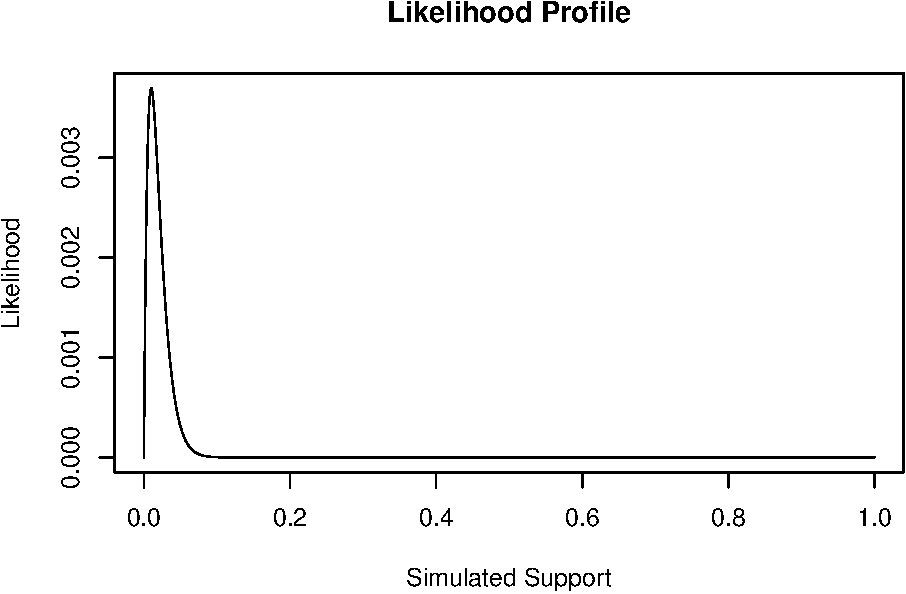
\includegraphics{lab-02_files/figure-latex/unnamed-chunk-3-1.pdf}

\end{document}
